\chapter{Introduction} % Write in your own chapter title
\label{Chapter1}
\lhead{} % Write in your own chapter title to set the page header

\section{Motivation}
% Motivate Deep Unfolding and Matrix Completion and in the end link the two. 
Deep unfolding is a recent approach that economizes on data and computational requirements yet solves optimization problems with impressive accuracy. This approach has an important advantage over traditional iterative algorithms in that it is more robust to perturbations in inputs and numerical errors. It also has one over traditional neural networks in that it has significantly lower data and computational requirements to perform reasonably. Matrix completion is a problem where a data set is missing some entries while the non-missing entries are possibly affected by noise. There are various iterative algorithms to solve this problem, but research employing unfolded algorithms has been scant.

\section{Problem Statement}
% Getting benefits of unrolling iterative algorithms to improve inference time and accuracy on datasets corrupted by impulsive GMM noise. 
Our objective is to reap the benefits of unfolded optimization algorithms, namely, faster inferences and higher accuracy scores, on data that has been corrupted by impulsive GMM noise.

\section{General Block Diagram}
% Provide high level diagram of convmc and hubermc and explain the pipeline. i.e. very concisely and briefly mention the matrix factorization vs the PCP formulation on which both are based
ConvMC-Net takes a single zero matrix as input with the goal to process it in a way that brings it as close to the original matrix as possible. The processing basically involves singular value thresholding (SVT), measurement matrices, and algebraic manipulation to create an update equation for a multi-layer neural network that finally outputs the recovered matrix.

ConvHuberMC-Net (shown in Figure \ref{fig:convhubermc_block}), on the other hand, follows a different approach. The model takes the corrupted matrix, perhaps some sensor data, as input, along with two other smaller matrices whose product has the same dimensions as the corrupted matrix. The smaller matrices are then processed via the Huber regression algorithm in each layer of the neural network, potentially being refined in a way that makes their product, the recovered matrix, reasonably similar to the pristine version of the corrupted matrix. Details for both ConvMC-Net and ConvHuberMC-Net in chapter 3. 

\begin{figure}
    \centering
    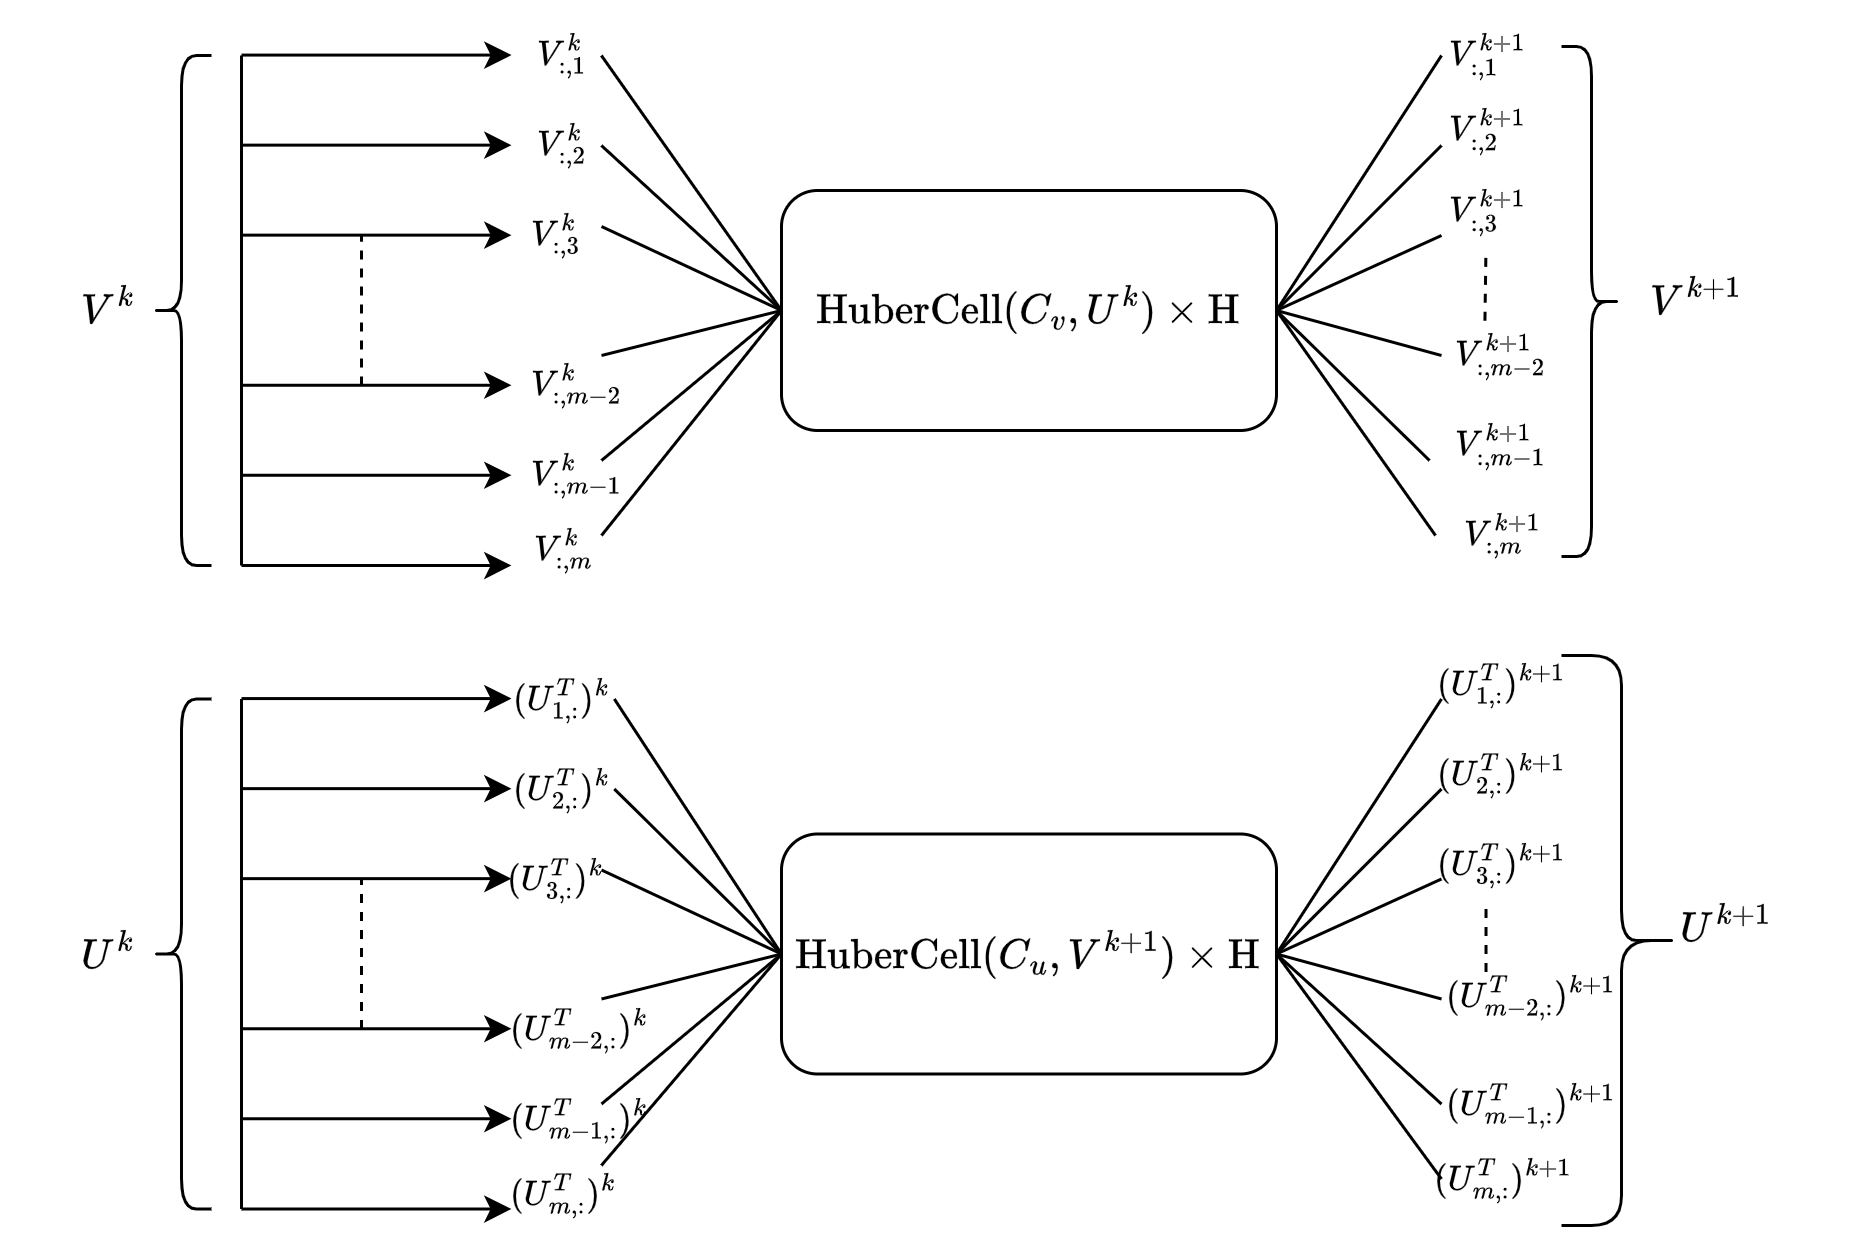
\includegraphics[scale=0.25]{HuberMC-Net}
    \caption{Block diagram of ConvHuberMC-Net}
    \label{fig:convhubermc_block}
\end{figure}

\section{Objectives}
The road map for developing the ideas proposed in this thesis consists of the following sequential objectives:
\begin{enumerate}
    \item Foundational knowledge regarding optimization and matrix completion from \cite{Wright-Ma-2022}.
    \item Identification of data sets related to this task, such as those of sensor networks or grayscale images.
    \item Review of other work done in the domains of matrix completion, compressed sensing, or deep unfolding (e.g., image generation using labelled segmentation maps).
    \item Design and implementation of a pipeline to help achieve our objectives.
\end{enumerate}

\section{Outcomes}
A desirable outcome of this research project is a proven capability to get seamless and accurate image reconstruction or wireless network node measurements or recommendation systems based on supervised methods. As far as social outcomes are considered, we hope that the ideas developed can be used relevant organizations for more accurate decision making.

\section{Outputs}
We intend to deliver a unfolded deep learning architecture that could be used for solving matrix completion problems in Pakistan and elsewhere. This may be presented as an open-source software or as a theoretical framework in a poster, thesis, or research paper.

\section{Timelines and the distribution of work}
% borrow content from compiled report shared with Sir before. 
% Expected:
% 1) Coursework and Preliminary Studies
% 2) Research and Experimentation and Replicating Results
% 3) Refining Shoaib Bhai's work (maybe add footnote here of the slump we faced during this time)
% 4) Literature Review
% 4) Experimenting and Comparing results with different algorithms on different datasets. 
% 5) Further refining pipeline until satisfactory results in most areas
% 6) Finalization
% Reality: 
% 4) Ideation
% 5) Literature Review
% 6) Detailed Experimentation on HuberMC
% 7) Finalization of Deliverables
We originally began this project in June 2023, starting off with an in-depth study of deep learning and signal processing. Eventually, we moved on to studying the work of Shoaib Imran (such as \cite{duparpca} and \cite{dustrpca}), including an incomplete paper and companion code on unfolding the augmented Lagrange multiplier (ALM) for matrix completion. This was the ConvMC-Net model. Our first actual task was to refine and complete the code, run experiments on synthetic and image data sets, compile the results, and compare them with those of existing matrix completion algorithms. Once this was done, the second task was to keep repeating this process until we had satisfactory performance over the two kinds of data sets. The final task was to document this improved performance in a research paper. However, only after we had compiled the results did we realize that our model makes a simplifying assumption: it assumes that the input matrix only has missing entries and is untouched by any kind of noise. Though this is a useful problem to solve in certain scenarios, it is quite limited in its capabilities compared to a model that can also deal with noise. At this point, we delved into the literature to see whether the assumption of noise can be incorporated into ALM and if not, then whether there exist other algorithms that can be unfolded for this task. We eventually settled on M-estimation, which led to our second model, ConvHuberMC-Net. From this point onward, we experimented extensively on several aspects of the new model and concluded with the results presented in this report. 

% \begin{figure}
%   \centering
%   \includegraphics{}
%   \caption{Timeline of the work}
%   \label{fig:timeline}
% \end{figure}